\documentclass{article}
\usepackage[margin=1.2in]{geometry}
\usepackage{parskip}
\usepackage{amsthm}
\usepackage{amssymb}
\usepackage{amsmath}
\usepackage{cite}
\usepackage{graphicx}
\usepackage{epsfig}
\pagestyle{plain}
\topmargin -0.8in
\textheight 9.0in
\oddsidemargin -0.1in
\textwidth 6.8in

\title{\textbf{CS697: Unsupervised Cross Lingual Alignment\\} Report}
\author{\normalsize Pranjal Singh 10327511\\
\emph{Indian Institute of Technology,Kanpur}\\ Advisor: Prof. Satyadev Nandakumar}

\date{\today}
\begin{document}
\maketitle
\begin{abstract}
The world today is full of large volumes of text resources spreading over internet, journals and digital libraries. These resources are present in almost all major languages. The main problem here is that texts may differ in two languages and there is a need that these should be aligned in all languages. This can be used to detect inconsistencies in the two texts. We present a framework which understands this problem of cross lingual alignment and tries to provide a solution for a very special set of problems where data is focused on only one topic. The data used is a manually built corpus in English and Hindi which is focused on only one topic, i.e., coal scam.
\end{abstract}

\section{Introduction}
With an ever increasing volume of text, there is a need that these should be connected in some way. This need can be easily understood by the example of Wikipedia. Wikipedia has very well grown into a multilingual resource containing information from every field. English has the largest wikipedia among all languages and the amount of information present in English wikipedia exceeds information present in any single wikipedia. This is mainly due to cultural and regional differences present across all languages, sometimes also called as cultural or regional bias. The need is to enrich each and every wikipedia so that every group of people come to know more about every other thing.\\\\
Same is the case with any electronic dictionary in medical domain, which are not properly connected. The word cross-lingual alignment in both these cases essentially means that corresponding lexicons in, say for example, two languages, English and Hindi, are directly connected or atleast have some semantic connection. For the ease of understanding, we will take only two languages in this work and in the coming sections we will discuss only these two languages, namely English and Hindi. \\
The problem of word-alignment is to find correspondence between words and phrases in parallel texts. Suppose we have two languages L1 and L2, then the task in hand is to identify which word token in L1 corresponds to which word token in L2.\\
For simplicity, as told above, we will take two languages, i.e., English and Hindi for describing examples. This can be extended to any pair of two languages.\\\\
The alignment of punctuation is also one of the important tasks but for now, the main focus are not the punctuations.
The difficulty is that we don't have a parallel corpora and is generally the most common scenario. Most of the work in cross-lingual alignment which has been done by today is mainly on a parallel corpora using tools such as GIZA++.\\
The rest of the text is organized as follows. Section 2 discusses some of the previous works which have been done in similar area. Section 3 discusses about the data which we will be using. Section 4 discusses about the Methodology which we have adopted. Section 5 discusses about the syntax of the final output and how can it be interpreted. Section 6 discusses about the Evaluation parameters which describe the extent of goodness of an alignment. Section 7 describes my previous work which is a basis of this work. Section 8 further discusses the limits of this work and what can be done in future. Section 9 acknowledges my advisor and Section 10 are the references for this work.

\section{Previous Work}
Most of the previous work in this area has been supervised and there is as such no currently existing work which looks into cross lingual alignment in great detail, mainly on a large corpus which contains all sought of information related to a topic.\\
There is a work called DbPedia (Auer et al., 2008) which is an ongoing, large project and it automatically extracts information from Wikipedia, normalizes the extracted information, links the information with other online data repositories and provides an interactive access.\\
It has been said that word alignment, like many other NLP tasks (Banko and Brill, 2001), highly improves if there is a large amount of training data available but then providing large amount of training data is also not trivial. This is due to the fact that different domains need different type of training data and different type of feature vectors. Currently, there is no general technique that can serve useful for different NLP tasks. However, there has been work in this direction where people are looking into general representations of tokens(Collobert and Weston, 2008) and (Bengio et. al, 2009) which can aid in almost all NLP tasks but still it lags in accuracy. They have been referred as embeddings.\\\\
The above work discusses unsupervised approach but nowadays there has been more focus on semi-supervised approaches where people are trying to improve existing baseline systems by introducing some unsupervision into them. Unsupervised word representations are pushed into existing systems and they try to improve upon their result(Turian, Retinov \& Bengio, 2010).\\
Recent days, there also has been focus on Lexical Substitution which aims to substitute target words(or phrases) in a context, which could prove very useful in paraphrasing and textual entailment. Apidianaki et al. has worked on Cross-Lingual lexical substitution where he has developed a framework that can substitute a target word in a context with several alternative substitute words in another language. The work is unsupervised and and exploits the results of a cross-lingual word sense induction method that derives the sense of the words by clustering their translations using their semantic similarity. The output of this work may prove to be an input to cross-lingual Information Retrieval and Machine Translation Systems (Sinha et al., 2009) and (Mihalcea et al., 2010).\\\\
There also have been various statistical techniques and alignment heuristics(Brown et al., 1993; Vogel et al., 1996; Melamed, 2000) which have looked into automatic alignment of words and phrases. These word alignment techniques generally contain links between multi-word units or phrases, where some of the lexical items cannot be separated into words which match in another language.

\begin{figure}[h!tb]
\centering
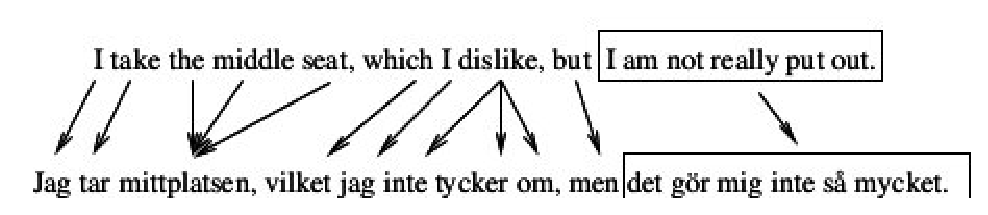
\includegraphics[width=8cm,height=2cm]{1.eps}
\caption {Example of word alignment from Saul Bellow "To Jerusalem and back: a personal account" (Bellow, 1976) and its Swedish translation (Bellow, 1977) (the \emph{Bellow Corpus})}
\end{figure}

Here, it can be easily seen that most of the words are properly connected to that in other language but the English unit "I am not really put out" doesn't have any proper way of connecting it to words in Swedish expression. So the whole expression is linked to the corresponding Swedish expression.\\
In some approaches, few complex expressions are separated in pre-processing step and later they are handled as complex units in the same ways as single words. This is very similar to the way ADIOS(Zach Solan, 2005) handles complex phrases and later treats them as single units. ADIOS can detect hidden syntactic units present in a large document which, in general, cannot be analysed just by looking into the document. It also summarizes the documents as few production rules which may serve useful in grammar induction.\\\\
Having discussed some previous work in this area, the next few sections will now describe how the current problem is formulated and how we can try to solve the problem.

\section{Data}
The data for this type of work can be any data which is focused on only one topic so that there is a a large correspondence between the tokens in both the languages.\\\\
For example, the data which was used in my previous work in CS498.\\
It is a manually built corpus on \emph{Coal Scam} in English and Hindi collected from various online Hindi and English newspaper and news channel websites such as \emph{Dainik Jagran, Hindustan, Aaj Tak}, etc. Hindi corpus has more than 35,000 tokens whereas English corpus has over 50,000 tokens. Stemming is to be ignored in this work to preserve syntax.\\\\
For evaluation, Gold Standard Word Aligned Data can be used with each annotator adding Certain and Probable tags to each aligned pair.\\

\section{Methodology}
\subsection{PLSA: Probabilistic Latent Semantic Analysis}
PLSA models co-occurrence information in a probabilistic framework which can discover the underlying semantic structure of the data. We have our corpus in term-document matrix form as input to this PLSA framework which extracts topics as clusters from it. PLSA considers the following three variables:
\begin{itemize}
\item Documents:$d \in D=\{d_1,d_2,....,d_N\}$ are the observed/visible variables where $N$ is the total number of documents given by the size of our corpus.
\item Words:$w \in W=\{w_1,w_2,...,w_M\}$ are again the observed variables where $M$ is the number of distinct words in the corpus.
\item Topics:$z \in Z=\{z_1,z_2,...,z_K\}$ are the latent/hidden variables where $K$ is to be assigned in advance. \\
\end{itemize}
PLSA models the following generative process:
\begin{itemize}
\item Select a document $d_n$ with probability $P(d)$
\item For every word $w_i, i \in {1,...,N_w}$ present in the document $d_n$:
\begin{itemize}
\item Choose a topic $z_i$ with probability $P(z|d_n)$ from a multinomial conditioned on the given document
\item Choose a word $w_i$ with probability $P(w|z_i)$ from a multinomial conditioned on the topic chosen previously\\
\end{itemize}
\end{itemize}

The predictive probability of PLSA model will be denoted by $P(w|d)$, and hence the objective function is given by:
\begin{center}
$L=\prod_{d,w}P(w|d)=\prod_{d \in D}\prod_{w \in W}P(w|d)^{n(d,w)}$
\end{center}
where $n(d,w)$ represents the frequencies observed, as in, the number of times word $w$ appears in document $d$.\\
Since, this turns out to be a non-convex optimization problem, it can be solved using EM(Expectation Maximization) algorithm.\\\\
PLSA uses EM-algorithm for following log-likelihood problem:\\
\begin{center}
$M=\log L=\prod_{d \in D}\prod_{w \in W}n(d,w).\log \sum_{z \in Z}P(w|z)P(z|d)$
\end{center}

\subsection{Formulation}

We have in hand two corpus which are basically focused on a single topic $Z$.\\
We have used Latent Topic Clustering and Unsupervised Syntax Induction Model of ADIOS to derive corresponding clusters in both the languages which have almost similar tokens in both the languages. These can serve as a ID to the corresponding lines in the two languages.\\
These can also serve as identifier to complex expressions which cannot be aligned word to word. So they are handled in pre-processing step (Smadja et al., 1996; Ahrenberg et al., 1998; Tiedemann, 1999).
\\\\
We plan to use the following three features of tokens for both languages:
\begin{enumerate}
\item Direct Mapping using bilingual dictionaries for same meaning tokens
\item Predicted Mapping using Clusters derived above
\item Semantic Mapping such as synonymy using Word-Net resource and POS tags in both the languages.
\end{enumerate}

The problem reduces to a matrix solving problem which is basically a Bag-of-Words Model and further can be converted into a \emph{tf-idf} model. Rows contain sentences in one language and column contains those in the other language. Each row element is itself a $n$-dimensional vector, where $n$ is the number of tokens in that sentence. We need to reorder rows and columns such that scores for each of the cell of the matrix maximizes.\\
A general representation for word-to-word alignment $L$ for a given cross-lingual text with $N$ words($a_1,a_2,...,a_N$) from one language and $M$ words($b_1,b_2,....,b_M$) from other language can be written as:\\ $L={L_1,L_2,...,L_p}, L_p=[a_{x_1},b_{x_2}],x_1 \in \{1,...,N\},x_2$\\\\
Direct mapping is certainly the best alignment and should be given the maximum score. Since predicted mapping take into account both semantics and syntax, its score will be less than direct mapping score. Semantic mapping score will also be less than direct mapping and will depend on the amount of semantic similarity present.\\
For semantic mapping, words can be extracted from English and Hindi WordNet. It can provide Synonym relation among words. Although this can be time consuming, but if each word in the corpus has an associated vector containing all \emph{*-nymy} relations in it from the very beginning, we can definitely save some time.

\section{Syntax}
The final word-aligned file will be a description of each word-to-word mapping with the corresponding line number. For example,\\
18 1 1\\
18 2 2\\\\
This means that word numbers 1 \& 2 in line numbers 18 of both the languages align with each other.\\
In addition, we can have two fields called Certain(C) and Probable(P) denoting the type of alignment. Certainty can vary between [0-1] adding another field which we will call as Accuracy(A).\\
\begin{itemize}
\item Items which are separated by a white space or a punctuation will be called a word. They are the ones which need to be aligned.
\item Any extra tokens which have no corresponding tokens in the other language will be substituted by COPY token which means, no subtraction in score for that.
\item Sometimes two lines may mean the same thing or a part of the line may mean the same, so the two sub-parts will be said as aligned.
\item Alignment scores will also be given when two numbers are aligned in both languages, say for example, when dates are aligned
\end{itemize}
The Gold standard alignment will also be scored against our current system so that we can assign proper scores.

\section{Evaluation}
Evaluation will be done using three different measures- Precision(P), Recall(R) and F-Score(F). Precision and recall have turned out to be quite useful in various NLP tasks, so we will be using them as our evaluation parameter.\\
We have alignment $A$ derived by our algorithm and $G$ is the Gold Standard Alignment.
\begin{align*}
&P_X=\frac{|A_X \cap G_X|}{A_X}\\
&R_X=\frac{|A_X \cap G_X|}{G_X}\\
&F_X=\frac{2P_XR_X}{P_X+R_X}\\
\end{align*}
where X ={C,P}, C-Certain, P-Probable\\\\
Precision(also called positive predictive value) is the fraction of retrieved instances that are relevant.\\
Recall(also known as sensitivity) is the fraction of relevant instances that are retrieved.\\
F-Score is the \emph{harmonic mean} of precision and recall.


\section{Base Results/Motivation}
\begin{figure}[h!tb]
\centering
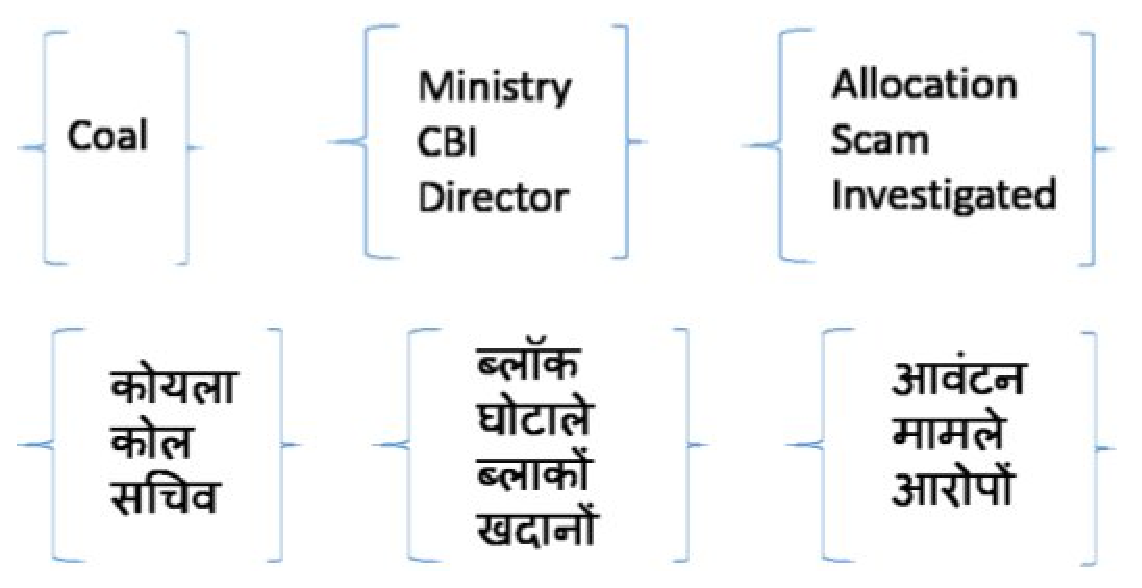
\includegraphics[width=8cm,height=4cm]{2.eps}
\caption {Cluster of size 3 obtained from PLSA technique which indicates cross lingual relationship between Hindi and English in our focused corpora on Coal Scam}
\end{figure}
\begin{figure}[h!tb]
\centering
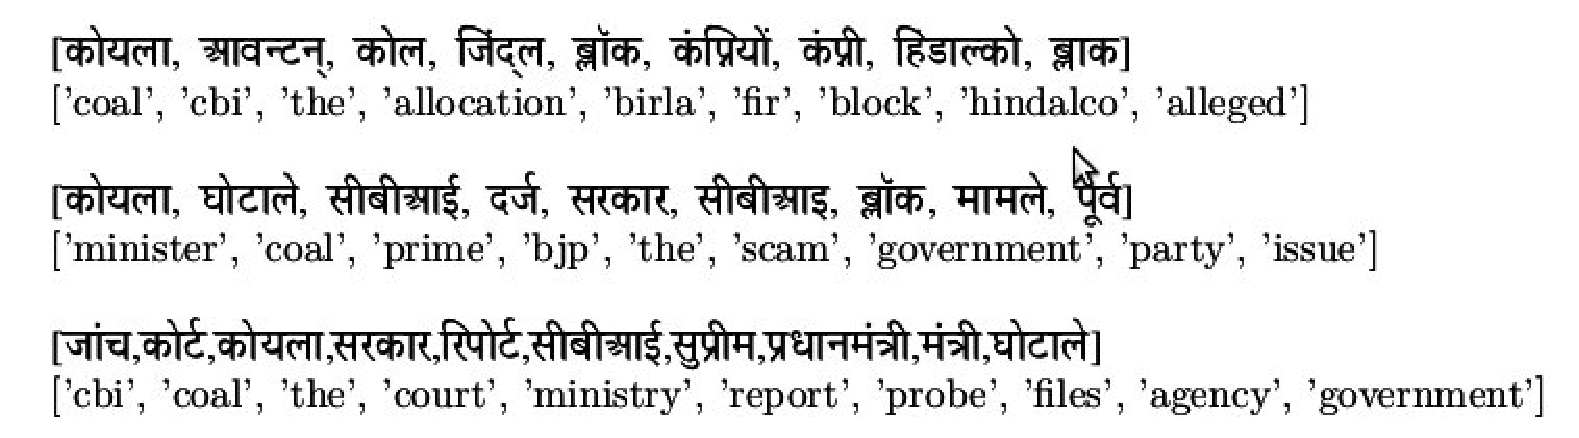
\includegraphics[width=11cm,height=4cm]{3.eps}
\caption {An output from ADIOS which again indicates cross lingual relationship between entities in Hindi and English in our focused corpora on Coal Scam}
\end{figure}

\newpage
\section{Future Work}
The quality of results can be easily improved if we use a large corpus though it slows down the rate of computing. We can also insert this unsupervised methodology into an existing supervised system and can improve its result. This would be more of a semi-supervised system.\\
We can also take into account phonemes for better alignment of tokens such as \emph{Nouns}. This work mainly describes a system for a focused corpora but it can be extended to work for a very general corpora.\\
We could also have tried working with n-gram clusters which could have provided better alignment for complex expressions.\\
We can also choose alignment strategies to suit particular needs.
We are re-ordering sentences in the corpus to align them in both languages but this may lead to loss of some semantic information because semantic information varies across various sentences.\\
Also, score of predicted mapping should vary depending on the tokens but our system cannot infer directly how to manage scoring for this case.
In future work, we can experiment with different set of languages, in particular, generalize this approach for any two set of languages.

\section{Acknowledgement}
I would like to show my sincere gratitude towards Prof. Satyadev Nandakumar, Computer Science and Engineering Department, IIT Kanpur for his motivation to do this work and becoming my advisor for this work. I would also like to thank my all friends who have helped me throughout this project. I would also like to thank CSE Department, IIT Kanpur for providing such as courses as CS697 where we figure out completely new objectives and try to strengthen our concepts related to the topic by reading existing papers.

\nocite{*}
\bibliography{report}{}
\bibliographystyle{plain}

\end{document}
